% REV01 Sun 27 Jun 2021 14:04:15 WIB
% START Tue 04 May 2021 13:55:16 WIB

\chapter{EFFECT IS GIVEN TO THE DOLLS’ DRESSMAKER’S DISCOVERY}

Mrs John Rokesmith sat at needlework in her neat little room, beside a
basket of neat little articles of clothing, which presented so much of
the appearance of being in the dolls’ dressmaker’s way of business, that
one might have supposed she was going to set up in opposition to Miss
Wren. Whether the Complete British Family Housewife had imparted sage
counsel anent them, did not appear, but probably not, as that cloudy
oracle was nowhere visible. For certain, however, Mrs John Rokesmith
stitched at them with so dexterous a hand, that she must have taken
lessons of somebody. Love is in all things a most wonderful teacher,
and perhaps love (from a pictorial point of view, with nothing on but
a thimble), had been teaching this branch of needlework to Mrs John
Rokesmith.

It was near John’s time for coming home, but as Mrs John was desirous to
finish a special triumph of her skill before dinner, she did not go out
to meet him. Placidly, though rather consequentially smiling, she sat
stitching away with a regular sound, like a sort of dimpled little
charming Dresden-china clock by the very best maker.

A knock at the door, and a ring at the bell. Not John; or Bella would
have flown out to meet him. Then who, if not John? Bella was asking
herself the question, when that fluttering little fool of a servant
fluttered in, saying, ‘Mr Lightwood!’

Oh good gracious!

Bella had but time to throw a handkerchief over the basket, when Mr
Lightwood made his bow. There was something amiss with Mr Lightwood, for
he was strangely grave and looked ill.

With a brief reference to the happy time when it had been his privilege
to know Mrs Rokesmith as Miss Wilfer, Mr Lightwood explained what was
amiss with him and why he came. He came bearing Lizzie Hexam’s earnest
hope that Mrs John Rokesmith would see her married.

Bella was so fluttered by the request, and by the short narrative he had
feelingly given her, that there never was a more timely smelling-bottle
than John’s knock. ‘My husband,’ said Bella; ‘I’ll bring him in.’

But, that turned out to be more easily said than done; for, the instant
she mentioned Mr Lightwood’s name, John stopped, with his hand upon the
lock of the room door.

‘Come up stairs, my darling.’

Bella was amazed by the flush in his face, and by his sudden turning
away. ‘What can it mean?’ she thought, as she accompanied him up stairs.

‘Now, my life,’ said John, taking her on his knee, ‘tell me all about
it.’

All very well to say, ‘Tell me all about it;’ but John was very much
confused. His attention evidently trailed off, now and then, even while
Bella told him all about it. Yet she knew that he took a great interest
in Lizzie and her fortunes. What could it mean?

‘You will come to this marriage with me, John dear?’

‘N--no, my love; I can’t do that.’

‘You can’t do that, John?’

‘No, my dear, it’s quite out of the question. Not to be thought of.’

‘Am I to go alone, John?’

‘No, my dear, you will go with Mr Lightwood.’

‘Don’t you think it’s time we went down to Mr Lightwood, John dear?’
Bella insinuated.

‘My darling, it’s almost time you went, but I must ask you to excuse me
to him altogether.’

‘You never mean, John dear, that you are not going to see him? Why, he
knows you have come home. I told him so.’

‘That’s a little unfortunate, but it can’t be helped. Unfortunate or
fortunate, I positively cannot see him, my love.’

Bella cast about in her mind what could be his reason for this
unaccountable behaviour; as she sat on his knee looking at him in
astonishment and pouting a little. A weak reason presented itself.

‘John dear, you never can be jealous of Mr Lightwood?’

‘Why, my precious child,’ returned her husband, laughing outright: ‘how
could I be jealous of him? Why should I be jealous of him?’

‘Because, you know, John,’ pursued Bella, pouting a little more, ‘though
he did rather admire me once, it was not my fault.’

‘It was your fault that I admired you,’ returned her husband, with a
look of pride in her, ‘and why not your fault that he admired you? But,
I jealous on that account? Why, I must go distracted for life, if I
turned jealous of every one who used to find my wife beautiful and
winning!’

‘I am half angry with you, John dear,’ said Bella, laughing a little,
‘and half pleased with you; because you are such a stupid old fellow,
and yet you say nice things, as if you meant them. Don’t be mysterious,
sir. What harm do you know of Mr Lightwood?’

‘None, my love.’

‘What has he ever done to you, John?’

‘He has never done anything to me, my dear. I know no more against
him than I know against Mr Wrayburn; he has never done anything to me;
neither has Mr Wrayburn. And yet I have exactly the same objection to
both of them.’

‘Oh, John!’ retorted Bella, as if she were giving him up for a bad job,
as she used to give up herself. ‘You are nothing better than a sphinx!
And a married sphinx isn’t a--isn’t a nice confidential husband,’ said
Bella, in a tone of injury.

‘Bella, my life,’ said John Rokesmith, touching her cheek, with a grave
smile, as she cast down her eyes and pouted again; ‘look at me. I want
to speak to you.’

‘In earnest, Blue Beard of the secret chamber?’ asked Bella, clearing
her pretty face.

‘In earnest. And I confess to the secret chamber. Don’t you remember
that you asked me not to declare what I thought of your higher qualities
until you had been tried?’

‘Yes, John dear. And I fully meant it, and I fully mean it.’

‘The time will come, my darling--I am no prophet, but I say so,--when
you WILL be tried. The time will come, I think, when you will undergo
a trial through which you will never pass quite triumphantly for me,
unless you can put perfect faith in me.’

‘Then you may be sure of me, John dear, for I can put perfect faith in
you, and I do, and I always, always will. Don’t judge me by a little
thing like this, John. In little things, I am a little thing myself--I
always was. But in great things, I hope not; I don’t mean to boast, John
dear, but I hope not!’

He was even better convinced of the truth of what she said than she was,
as he felt her loving arms about him. If the Golden Dustman’s riches had
been his to stake, he would have staked them to the last farthing on the
fidelity through good and evil of her affectionate and trusting heart.

‘Now, I’ll go down to, and go away with, Mr Lightwood,’ said Bella,
springing up. ‘You are the most creasing and tumbling Clumsy-Boots of a
packer, John, that ever was; but if you’re quite good, and will promise
never to do so any more (though I don’t know what you have done!) you
may pack me a little bag for a night, while I get my bonnet on.’

He gaily complied, and she tied her dimpled chin up, and shook her head
into her bonnet, and pulled out the bows of her bonnet-strings, and
got her gloves on, finger by finger, and finally got them on her
little plump hands, and bade him good-bye and went down. Mr Lightwood’s
impatience was much relieved when he found her dressed for departure.

‘Mr Rokesmith goes with us?’ he said, hesitating, with a look towards
the door.

‘Oh, I forgot!’ replied Bella. ‘His best compliments. His face is
swollen to the size of two faces, and he is to go to bed directly, poor
fellow, to wait for the doctor, who is coming to lance him.’

‘It is curious,’ observed Lightwood, ‘that I have never yet seen Mr
Rokesmith, though we have been engaged in the same affairs.’

‘Really?’ said the unblushing Bella.

‘I begin to think,’ observed Lightwood, ‘that I never shall see him.’

‘These things happen so oddly sometimes,’ said Bella with a steady
countenance, ‘that there seems a kind of fatality in them. But I am
quite ready, Mr Lightwood.’

They started directly, in a little carriage that Lightwood had brought
with him from never-to-be-forgotten Greenwich; and from Greenwich they
started directly for London; and in London they waited at a railway
station until such time as the Reverend Frank Milvey, and Margaretta
his wife, with whom Mortimer Lightwood had been already in conference,
should come and join them.

That worthy couple were delayed by a portentous old parishioner of the
female gender, who was one of the plagues of their lives, and with whom
they bore with most exemplary sweetness and good-humour, notwithstanding
her having an infection of absurdity about her, that communicated itself
to everything with which, and everybody with whom, she came in contact.
She was a member of the Reverend Frank’s congregation, and made a point
of distinguishing herself in that body, by conspicuously weeping at
everything, however cheering, said by the Reverend Frank in his public
ministration; also by applying to herself the various lamentations of
David, and complaining in a personally injured manner (much in arrear of
the clerk and the rest of the respondents) that her enemies were digging
pit-falls about her, and breaking her with rods of iron. Indeed, this
old widow discharged herself of that portion of the Morning and Evening
Service as if she were lodging a complaint on oath and applying for
a warrant before a magistrate. But this was not her most inconvenient
characteristic, for that took the form of an impression, usually
recurring in inclement weather and at about daybreak, that she had
something on her mind and stood in immediate need of the Reverend Frank
to come and take it off. Many a time had that kind creature got up, and
gone out to Mrs Sprodgkin (such was the disciple’s name), suppressing
a strong sense of her comicality by his strong sense of duty, and
perfectly knowing that nothing but a cold would come of it. However,
beyond themselves, the Reverend Frank Milvey and Mrs Milvey seldom
hinted that Mrs Sprodgkin was hardly worth the trouble she gave; but
both made the best of her, as they did of all their troubles.

This very exacting member of the fold appeared to be endowed with a
sixth sense, in regard of knowing when the Reverend Frank Milvey least
desired her company, and with promptitude appearing in his little hall.
Consequently, when the Reverend Frank had willingly engaged that he and
his wife would accompany Lightwood back, he said, as a matter of course:
‘We must make haste to get out, Margaretta, my dear, or we shall be
descended on by Mrs Sprodgkin.’ To which Mrs Milvey replied, in her
pleasantly emphatic way, ‘Oh YES, for she IS such a marplot, Frank, and
DOES worry so!’ Words that were scarcely uttered when their theme
was announced as in faithful attendance below, desiring counsel on a
spiritual matter. The points on which Mrs Sprodgkin sought elucidation
being seldom of a pressing nature (as Who begat Whom, or some
information concerning the Amorites), Mrs Milvey on this special
occasion resorted to the device of buying her off with a present of tea
and sugar, and a loaf and butter. These gifts Mrs Sprodgkin accepted,
but still insisted on dutifully remaining in the hall, to curtsey to the
Reverend Frank as he came forth. Who, incautiously saying in his genial
manner, ‘Well, Sally, there you are!’ involved himself in a discursive
address from Mrs Sprodgkin, revolving around the result that she
regarded tea and sugar in the light of myrrh and frankincense, and
considered bread and butter identical with locusts and wild honey.
Having communicated this edifying piece of information, Mrs Sprodgkin
was left still unadjourned in the hall, and Mr and Mrs Milvey hurried in
a heated condition to the railway station. All of which is here recorded
to the honour of that good Christian pair, representatives of hundreds
of other good Christian pairs as conscientious and as useful, who merge
the smallness of their work in its greatness, and feel in no danger of
losing dignity when they adapt themselves to incomprehensible humbugs.

‘Detained at the last moment by one who had a claim upon me,’ was the
Reverend Frank’s apology to Lightwood, taking no thought of himself.
To which Mrs Milvey added, taking thought for him, like the championing
little wife she was; ‘Oh yes, detained at the last moment. But AS to
the claim, Frank, I MUST say that I DO think you are OVER-considerate
sometimes, and allow THAT to be a LITTLE abused.’

Bella felt conscious, in spite of her late pledge for herself, that her
husband’s absence would give disagreeable occasion for surprise to the
Milveys. Nor could she appear quite at her ease when Mrs Milvey asked:

‘HOW is Mr Rokesmith, and IS he gone before us, or DOES he follow us?’

It becoming necessary, upon this, to send him to bed again and hold him
in waiting to be lanced again, Bella did it. But not half as well on
the second occasion as on the first; for, a twice-told white one seems
almost to become a black one, when you are not used to it.

‘Oh DEAR!’ said Mrs Milvey, ‘I am SO sorry! Mr Rokesmith took SUCH an
interest in Lizzie Hexam, when we were there before. And if we had ONLY
known of his face, we COULD have given him something that would have
kept it down long enough for so SHORT a purpose.’

By way of making the white one whiter, Bella hastened to stipulate that
he was not in pain. Mrs Milvey was SO glad of it.

‘I don’t know HOW it is,’ said Mrs Milvey, ‘and I am SURE you don’t,
Frank, but the clergy and their wives seem to CAUSE swelled faces.
Whenever I take notice of a child in the school, it seems to me as if
its face swelled INSTANTLY. Frank NEVER makes acquaintance with a new
old woman, but she gets the face-ache. And another thing is, we DO make
the poor children sniff so. I don’t know HOW we do it, and I should
be so glad not to; but the MORE we take notice of them, the MORE they
sniff. Just as they do when the text is given out.--Frank, that’s a
schoolmaster. I have seen him somewhere.’

The reference was to a young man of reserved appearance, in a coat and
waistcoat of black, and pantaloons of pepper and salt. He had come
into the office of the station, from its interior, in an unsettled way,
immediately after Lightwood had gone out to the train; and he had been
hurriedly reading the printed bills and notices on the wall. He had had
a wandering interest in what was said among the people waiting there
and passing to and fro. He had drawn nearer, at about the time when
Mrs Milvey mentioned Lizzie Hexam, and had remained near, since: though
always glancing towards the door by which Lightwood had gone out. He
stood with his back towards them, and his gloved hands clasped behind
him. There was now so evident a faltering upon him, expressive of
indecision whether or no he should express his having heard himself
referred to, that Mr Milvey spoke to him.

‘I cannot recall your name,’ he said, ‘but I remember to have seen you
in your school.’

‘My name is Bradley Headstone, sir,’ he replied, backing into a more
retired place.

‘I ought to have remembered it,’ said Mr Milvey, giving him his hand. ‘I
hope you are well? A little overworked, I am afraid?’

‘Yes, I am overworked just at present, sir.’

‘Had no play in your last holiday time?’

‘No, sir.’

‘All work and no play, Mr Headstone, will not make dulness, in your
case, I dare say; but it will make dyspepsia, if you don’t take care.’

‘I will endeavour to take care, sir. Might I beg leave to speak to you,
outside, a moment?’

‘By all means.’

It was evening, and the office was well lighted. The schoolmaster, who
had never remitted his watch on Lightwood’s door, now moved by another
door to a corner without, where there was more shadow than light; and
said, plucking at his gloves:

‘One of your ladies, sir, mentioned within my hearing a name that I am
acquainted with; I may say, well acquainted with. The name of the sister
of an old pupil of mine. He was my pupil for a long time, and has got on
and gone upward rapidly. The name of Hexam. The name of Lizzie Hexam.’
He seemed to be a shy man, struggling against nervousness, and spoke in
a very constrained way. The break he set between his last two sentences
was quite embarrassing to his hearer.

‘Yes,’ replied Mr Milvey. ‘We are going down to see her.’

‘I gathered as much, sir. I hope there is nothing amiss with the sister
of my old pupil? I hope no bereavement has befallen her. I hope she is
in no affliction? Has lost no--relation?’

Mr Milvey thought this a man with a very odd manner, and a dark downward
look; but he answered in his usual open way.

‘I am glad to tell you, Mr Headstone, that the sister of your old pupil
has not sustained any such loss. You thought I might be going down to
bury some one?’

‘That may have been the connexion of ideas, sir, with your clerical
character, but I was not conscious of it.--Then you are not, sir?’

A man with a very odd manner indeed, and with a lurking look that was
quite oppressive.

‘No. In fact,’ said Mr Milvey, ‘since you are so interested in the
sister of your old pupil, I may as well tell you that I am going down to
marry her.’

The schoolmaster started back.

‘Not to marry her, myself,’ said Mr Milvey, with a smile, ‘because I
have a wife already. To perform the marriage service at her wedding.’

Bradley Headstone caught hold of a pillar behind him. If Mr Milvey knew
an ashy face when he saw it, he saw it then.

‘You are quite ill, Mr Headstone!’

‘It is not much, sir. It will pass over very soon. I am accustomed to be
seized with giddiness. Don’t let me detain you, sir; I stand in need
of no assistance, I thank you. Much obliged by your sparing me these
minutes of your time.’

As Mr Milvey, who had no more minutes to spare, made a suitable reply
and turned back into the office, he observed the schoolmaster to
lean against the pillar with his hat in his hand, and to pull at his
neckcloth as if he were trying to tear it off. The Reverend Frank
accordingly directed the notice of one of the attendants to him, by
saying: ‘There is a person outside who seems to be really ill, and to
require some help, though he says he does not.’

Lightwood had by this time secured their places, and the departure-bell
was about to be rung. They took their seats, and were beginning to
move out of the station, when the same attendant came running along the
platform, looking into all the carriages.

‘Oh! You are here, sir!’ he said, springing on the step, and holding
the window-frame by his elbow, as the carriage moved. ‘That person you
pointed out to me is in a fit.’

‘I infer from what he told me that he is subject to such attacks. He
will come to, in the air, in a little while.’

He was took very bad to be sure, and was biting and knocking about him
(the man said) furiously. Would the gentleman give him his card, as he
had seen him first? The gentleman did so, with the explanation that
he knew no more of the man attacked than that he was a man of a very
respectable occupation, who had said he was out of health, as his
appearance would of itself have indicated. The attendant received the
card, watched his opportunity for sliding down, slid down, and so it
ended.

Then, the train rattled among the house-tops, and among the ragged sides
of houses torn down to make way for it, and over the swarming streets,
and under the fruitful earth, until it shot across the river: bursting
over the quiet surface like a bomb-shell, and gone again as if it had
exploded in the rush of smoke and steam and glare. A little more, and
again it roared across the river, a great rocket: spurning the watery
turnings and doublings with ineffable contempt, and going straight to
its end, as Father Time goes to his. To whom it is no matter what living
waters run high or low, reflect the heavenly lights and darknesses,
produce their little growth of weeds and flowers, turn here, turn there,
are noisy or still, are troubled or at rest, for their course has one
sure termination, though their sources and devices are many.

Then, a carriage ride succeeded, near the solemn river, stealing away
by night, as all things steal away, by night and by day, so quietly
yielding to the attraction of the loadstone rock of Eternity; and the
nearer they drew to the chamber where Eugene lay, the more they feared
that they might find his wanderings done. At last they saw its dim light
shining out, and it gave them hope: though Lightwood faltered as he
thought: ‘If he were gone, she would still be sitting by him.’

But he lay quiet, half in stupor, half in sleep. Bella, entering with
a raised admonitory finger, kissed Lizzie softly, but said not a word.
Neither did any of them speak, but all sat down at the foot of the bed,
silently waiting. And now, in this night-watch, mingling with the flow
of the river and with the rush of the train, came the questions into
Bella’s mind again: What could be in the depths of that mystery of
John’s? Why was it that he had never been seen by Mr Lightwood, whom he
still avoided? When would that trial come, through which her faith
in, and her duty to, her dear husband, was to carry her, rendering him
triumphant? For, that had been his term. Her passing through the trial
was to make the man she loved with all her heart, triumphant. Term not
to sink out of sight in Bella’s breast.

Far on in the night, Eugene opened his eyes. He was sensible, and said
at once: ‘How does the time go? Has our Mortimer come back?’

Lightwood was there immediately, to answer for himself. ‘Yes, Eugene,
and all is ready.’

‘Dear boy!’ returned Eugene with a smile, ‘we both thank you heartily.
Lizzie, tell them how welcome they are, and that I would be eloquent if
I could.’

‘There is no need,’ said Mr Milvey. ‘We know it. Are you better, Mr
Wrayburn?’

‘I am much happier,’ said Eugene.

‘Much better too, I hope?’

Eugene turned his eyes towards Lizzie, as if to spare her, and answered
nothing.

Then, they all stood around the bed, and Mr Milvey, opening his book,
began the service; so rarely associated with the shadow of death; so
inseparable in the mind from a flush of life and gaiety and hope and
health and joy. Bella thought how different from her own sunny little
wedding, and wept. Mrs Milvey overflowed with pity, and wept too. The
dolls’ dressmaker, with her hands before her face, wept in her golden
bower. Reading in a low clear voice, and bending over Eugene, who kept
his eyes upon him, Mr Milvey did his office with suitable simplicity.
As the bridegroom could not move his hand, they touched his fingers with
the ring, and so put it on the bride. When the two plighted their troth,
she laid her hand on his and kept it there. When the ceremony was done,
and all the rest departed from the room, she drew her arm under his
head, and laid her own head down upon the pillow by his side.

‘Undraw the curtains, my dear girl,’ said Eugene, after a while, ‘and
let us see our wedding-day.’

The sun was rising, and his first rays struck into the room, as she came
back, and put her lips to his. ‘I bless the day!’ said Eugene. ‘I bless
the day!’ said Lizzie.

‘You have made a poor marriage of it, my sweet wife,’ said Eugene. ‘A
shattered graceless fellow, stretched at his length here, and next to
nothing for you when you are a young widow.’

‘I have made the marriage that I would have given all the world to dare
to hope for,’ she replied.

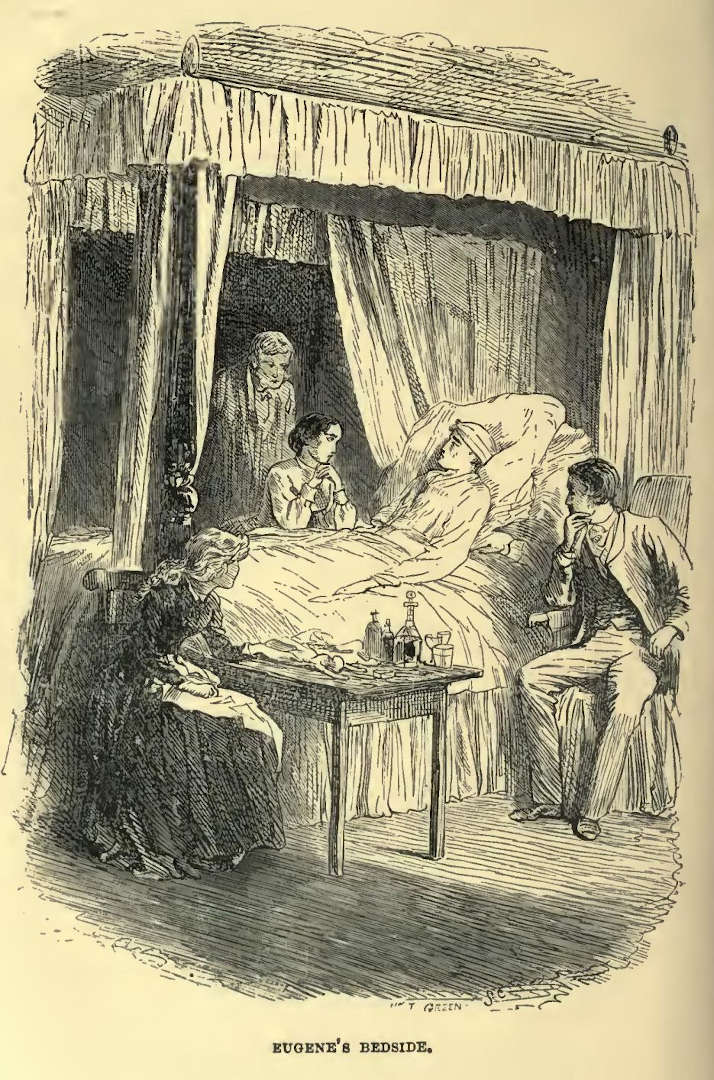
\includegraphics[scale=2.3]{04-11-01}

‘You have thrown yourself away,’ said Eugene, shaking his head. ‘But you
have followed the treasure of your heart. My justification is, that you
had thrown that away first, dear girl!’

‘No. I had given it to you.’

‘The same thing, my poor Lizzie!’

‘Hush! hush! A very different thing.’

There were tears in his eyes, and she besought him to close them. ‘No,’
said Eugene, again shaking his head; ‘let me look at you, Lizzie, while
I can. You brave devoted girl! You heroine!’

Her own eyes filled under his praises. And when he mustered strength to
move his wounded head a very little way, and lay it on her bosom, the
tears of both fell.

‘Lizzie,’ said Eugene, after a silence: ‘when you see me wandering away
from this refuge that I have so ill deserved, speak to me by my name,
and I think I shall come back.’

‘Yes, dear Eugene.’

‘There!’ he exclaimed, smiling. ‘I should have gone then, but for that!’

A little while afterwards, when he appeared to be sinking into
insensibility, she said, in a calm loving voice: ‘Eugene, my dear
husband!’ He immediately answered: ‘There again! You see how you can
recall me!’ And afterwards, when he could not speak, he still answered
by a slight movement of his head upon her bosom.

The sun was high in the sky, when she gently disengaged herself to give
him the stimulants and nourishment he required. The utter helplessness
of the wreck of him that lay cast ashore there, now alarmed her, but he
himself appeared a little more hopeful.

‘Ah, my beloved Lizzie!’ he said, faintly. ‘How shall I ever pay all I
owe you, if I recover!’

‘Don’t be ashamed of me,’ she replied, ‘and you will have more than paid
all.’

‘It would require a life, Lizzie, to pay all; more than a life.’

‘Live for that, then; live for me, Eugene; live to see how hard I will
try to improve myself, and never to discredit you.’

‘My darling girl,’ he replied, rallying more of his old manner than
he had ever yet got together. ‘On the contrary, I have been thinking
whether it is not the best thing I can do, to die.’

‘The best thing you can do, to leave me with a broken heart?’

‘I don’t mean that, my dear girl. I was not thinking of that. What I was
thinking of was this. Out of your compassion for me, in this maimed and
broken state, you make so much of me--you think so well of me--you love
me so dearly.’

‘Heaven knows I love you dearly!’

‘And Heaven knows I prize it! Well. If I live, you’ll find me out.’

‘I shall find out that my husband has a mine of purpose and energy, and
will turn it to the best account?’

‘I hope so, dearest Lizzie,’ said Eugene, wistfully, and yet somewhat
whimsically. ‘I hope so. But I can’t summon the vanity to think so. How
can I think so, looking back on such a trifling wasted youth as mine! I
humbly hope it; but I daren’t believe it. There is a sharp misgiving
in my conscience that if I were to live, I should disappoint your good
opinion and my own--and that I ought to die, my dear!’



